% This version of CVPR template is provided by Ming-Ming Cheng.
% Please leave an issue if you found a bug:
% https://github.com/MCG-NKU/CVPR_Template.

\documentclass[final]{cvpr}

\usepackage{times}
\usepackage{epsfig}
\usepackage{graphicx}
\usepackage{amsmath}
\usepackage{amssymb}
\usepackage[numbers]{natbib}
\usepackage{notoccite}
\usepackage{subcaption}
\captionsetup{compatibility=false}
\usepackage{graphicx}
\usepackage{fancyvrb}


% Include other packages here, before hyperref.

% If you comment hyperref and then uncomment it, you should delete
% egpaper.aux before re-running latex.  (Or just hit 'q' on the first latex
% run, let it finish, and you should be clear).
\usepackage[pagebackref=true,breaklinks=true,colorlinks,bookmarks=false]{hyperref}


\def\cvprPaperID{34} % *** Enter the CVPR Paper ID here
\def\confYear{CVPR 2021}
%\setcounter{page}{4321} % For final version only


\begin{document}
	
	%%%%%%%%% TITLE
	\title{Classification of Lymphocytosis from Blood Cells\\
		\vspace{1mm}
		\large \normalfont Deep Learning for Medical Imaging}
	
	\author{\textbf{Clément Grisi}\\
		École des Ponts ParisTech\\
		\small \url{grisi.clement@gmail.com}
	\and
	\textbf{Marius Schmidt-Mengin}\\
	École des Ponts ParisTech\\
	\small \url{marius.schmidt.mengin@gmail.com}
	}
	
	\maketitle
	
	\begin{abstract}
		In this report, we emphasize our work for the data challenge organized as part of the Deep Learning for Medical Imaging class. The goal of the challenge is to classify lymphocytosis from blood cells. Through iterations in model definition and data representation, we managed to get $0.96623$ classification accuracy on the academic leaderboard (rank 1).
	\end{abstract}
	
	\vspace{-3mm}
	
	\section{Introduction}
	
	Lymphocytosis is an increase in the number or proportion of lymphocytes in the blood. It's a common finding, which can be either a reaction to infection or acute stress (reactive), or the manifestation of a lymphoproliferative disorder -- a type of cancer of the lymphocytes (tumoral). In clinical practice, the diagnosis as either reactive or tumoral is performed by trained pathologists who visually inspect blood cells under a microscope. The final decision also takes into consideration clinical attributes such as age, gender, and lymphocyte count. In spite of being relatively fast and affordable, lymphocytosis diagnisis lacks reproducibility between experts. Additional clinical tests are often required to confirm the malignant nature of the lymphocytes. However, this analysis is relatively expensive and time-consuming, and therefore is not performed for every patient in practice. In this context, automatic classification has the potential to provide accurate and reproducible diagnosis, saving precious time and ressources by quickly identifying which patient should be referred for flow cytometry analysis.
	
	\section{Problem Definiton}
	
	\subsection{Dataset}
	
	Blood smears and patient attributes were collected from $204$ patients from the routine hematology laboratory of the Lyon SudUniversity Hospital. All included patients have a lymphocyte count above $4\times10^9/L$. The blood smears were automatically produced by a Sysmex automat tool, and the nucleated cells were automatically photographed with a DM-96 device. The training set consists of $142$ patients ($44$ reactive and $98$ malignant cases), and the testing set of $42$ patients. For each patient, we have access to dozens of images of lymphocytes, as well as the following clinical attributes: gender, age, and lymphocyte count.
	
	\subsection{Evalutation Metric} 
	
	This challenge is evaluated on balanced accuracy (BA), which normalizes true positive (TP) and true negative (TN) predictions by the number of positive and negative samples, respectively. In particular, if one denotes false positives as FP and false negatives as FN, we have:
	
	\vspace{-2mm}
	
	\begin{equation*}
		\begin{aligned}
			\text{Sensitivity} & = \dfrac{\text{TP}}{\text{TP}+\text{FN}} ,\quad 
			\text{Specificity} & = \dfrac{\text{TN}}{\text{TN}+\text{FP}}\\
		\end{aligned}
	\end{equation*}

	\begin{equation*}
		\begin{aligned}
			\text{BA} = \dfrac{\text{Sensitivity}+\text{Specificity}}{2}
		\end{aligned}
	\end{equation*}
		
	\vspace{2mm}
	
	\subsection{Weak Supervision through Multiple Instance Learning} 
	
	The idea of weakly supervised learning is to exploit coarse-grained annotations to automatically infer finer-grained information. Coarse-grained information is often readily available in the form of patient level labels, but finer grained annotations are more difficult to obtain. Without precise local annotations, classification models cannot be trained in a fully supervised manner. Therefore, various weakly supervised techniques have recently been developed to overcome this issue. One of these techniques relies on multiple instance learning (MIL), an existing framework largely used in classic computer vision that has recently showed state-of-the-art results in several medical imaging tasks \cite{hou_MIL}. \\
	\\
	Babenko \cite{mil} gives a good example to understand multiple instance learning. Imagine several people, each of them having a key chain that contains a few keys. Some of these people are able to enter a certain room, and some aren’t. The task is to predict whether or not a given key chain can open the door of that room. To solve this problem, one needs to find the exact key that is common to all the \textit{positive} key chains. If one can correctly identify this key, one can also correctly classify an entire key chain - \textit{positive} if it contains the required key, or \textit{negative} if it doesn't.\\
	\\
	Hence, the multiple instance learning framework allows the training of a classifier from weakly labeled data: instead of providing input-label pairs, labels $\ell_b$ are assigned to \emph{sets} or \emph{bags} of instances. In this setting, the true instance labels $\ell_i$ can be thought of as latent variables, as they are not known during training. In our case, we can assume that only a subset of the images available for a patient with tumoral lymphocytosis do carry the information necessary to correctly classify that patient. Identifying these special instances perfectly fits in the multiple instance learning framework.
	
	\section{Related Work}
	
	\section{Methodology}
	
	\subsection{Standard MIL Assumption} 
	
	top-$k$ = 1

	\subsection{Extended  MIL Assumption} 
	
	top-$k$ = hyperparameter

	\subsection{Towards a Custom Aggregation Function}
	
	top-$k$ \& bottom-$k$
	
	\subsection{Custom Aggregation  Function}
	
	taking all instances into consideration
	
	\section{Architecture}
	We adopt a simple architecture composed of a ResNet backbone followed by an aggregation module.
	All images are first passed independently through the backbone. The resulting features are then rearranged into different patients and passed through the aggregation module.
	As the number of images passed through the backbone is often large, we keep the gradients for only a subset of these images. Pseudo-code for this is provided by Algorithm 1.
	
	\begin{Verbatim}[fontsize=\footnotesize, samepage=true]
B, 3, H, W = image_batch.shape
max_forward_size = 512
max_backward_size = 512
features = []
i = 0
# forward images without keeping gradients
with torch.no_grad():
  while i < B - max_backward_size:
    j = min(i+max_forward_size,
            num_images-max_backward_size)
    features.append(backbone(images[i:j]))
    i = j
# forward image with gradients
features.append(backbone(images[i:]))
	\end{Verbatim}

\begin{figure}[t]
	\begin{center}
		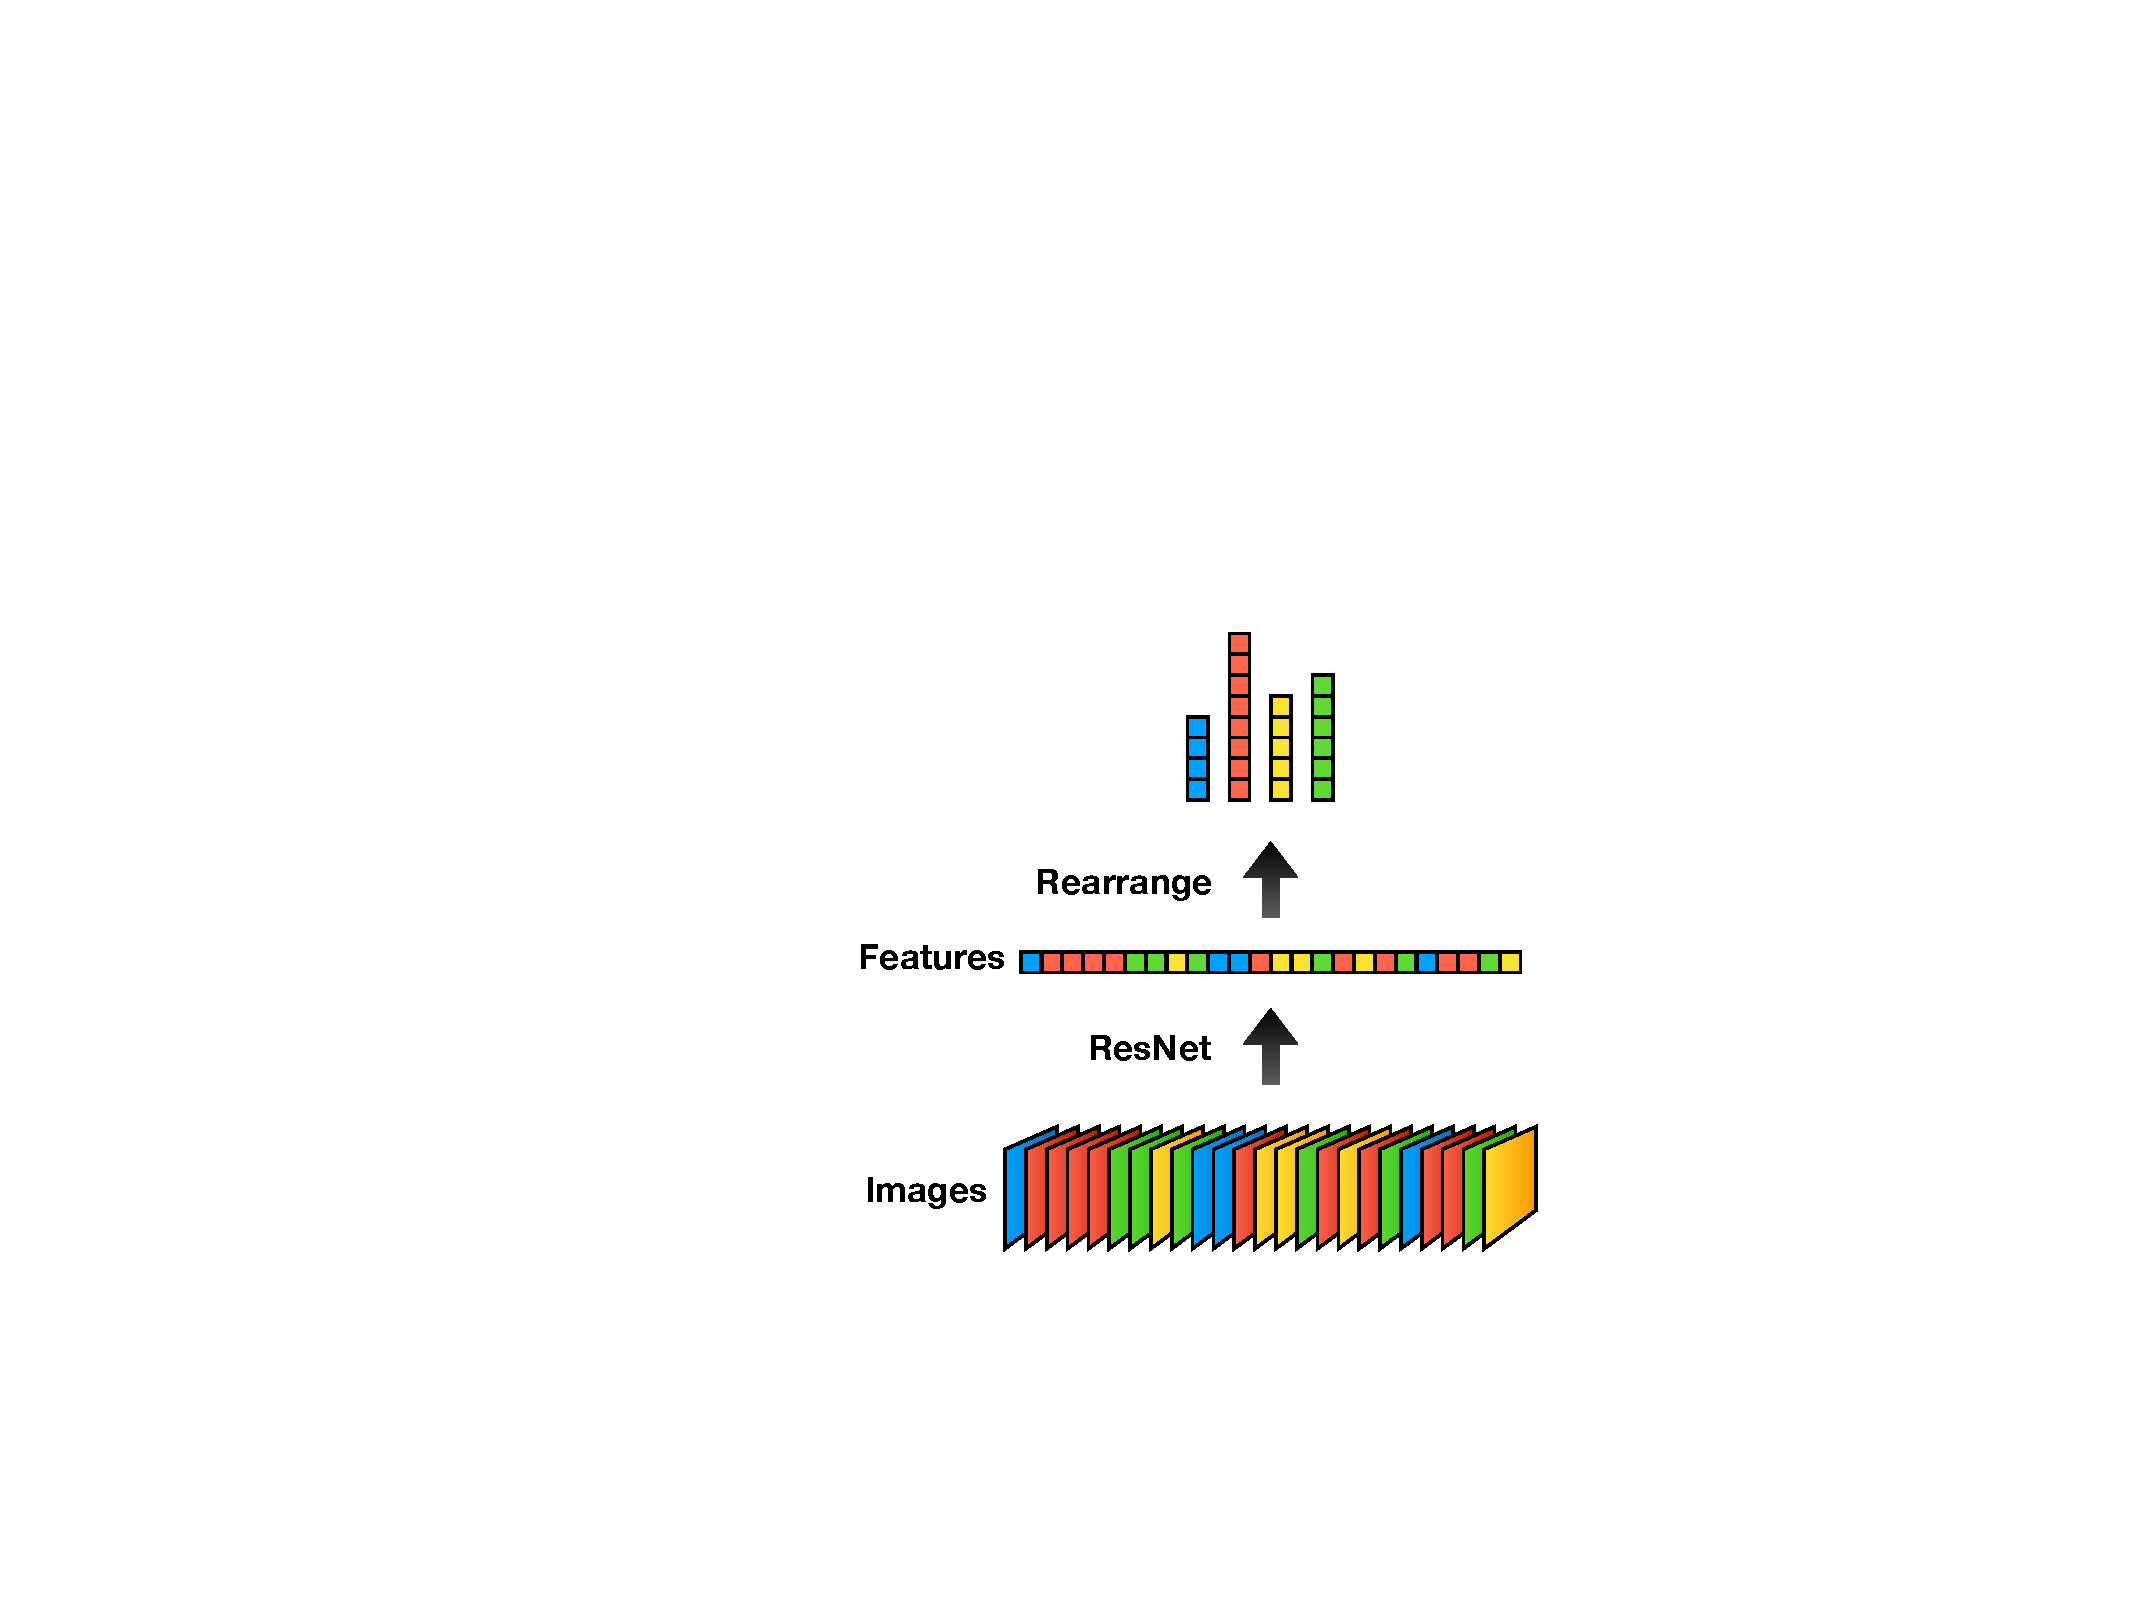
\includegraphics[width=0.9\linewidth]{graphic.pdf}
	\end{center}
	\caption{Overview.}
	\label{fig:overview}
\end{figure}
	
	\section{Results}
	
	\section{Conclusion}
	
	
	{\small
		\bibliographystyle{unsrt}
		\bibliography{egbib}
	}

\end{document}